\chapter{Background}
\label{bckgnd}

\section{ Machine Learning}
Machine learning is the field of computer science that allows computers to acquire knowledge from data and make some sort of prediction or estimation without explicitly programming that knowledge \cite{bishop_2013}. \citet{ai_text_book} say that a machine learning algorithm is designed for a particular task or problem, and is learning if it improves its performance at that task depending on a metric. Machine learning is useful for tasks that require pattern recognition, especially in large amounts of data.  Examples of such tasks include handwriting recognition, cybersecurity breach detection, medical disease diagnosis and autonomous cars control systems \cite{lecun1998mnist,cybersecurity,3d_conf_for_alzheimers,driverless_cars}. Due to the variety of tasks that could fit this broad definition, there are also a variety of approaches that we could use to solve each of those particular tasks.


\subsection{Supervised Learning}
\label{supervised}

Supervised learning is a task that tries to learn a model that maps from a domain of inputs to a range of outputs using data on which the task has already been accomplished by humans. Mathematically, if $\mathcal{S} =\{ ( \mathbf{X_i}, \mathbf{y_i} ) \ | \ i = 1...N\} \subset \mathcal{P}$, then the machine learning task may be to find a function, $ \mathbf{\hat{y}} = f(\mathbf{X}) $, an estimate of $\mathbf{y}$ for any $(\mathbf{X}, \mathbf{y}) \in \mathcal{P}$ where $\mathbf{X}$ is an input, $\mathbf{y}$ is an output (the label or a target), $\mathbf{\hat{y}}$  is an estimate of the output from the machine learning model, $\mathcal{S}$ is the training set of $N$ examples of input-output pairs, and $\mathcal{P}$ is the population of input-output pairs. 

\noindent
For example, in the case of the hand-written digits recognition using the data provided by \citet{lecun1998mnist}, the input $\mathbf{X}$ may be the image of the digit, $\mathbf{y}$ will be the true label of the digit provided by the dataset, and $\mathbf{\hat{y}}$ is the discrete value that the algorithm infers restricted to the range of $\mathbf{y}$. This particular process is called classification since we are restricted to a discrete set of values that are predefined. In order to learn a mapping from $\mathbf{X}$ to $\mathbf{y}$, a loss function, $J(\mathbf{y}, \mathbf{\hat{y}})$, can be used to quantify how well our model performs on our sample set, $\mathcal{S}$. In supervised learning, $J(\mathbf{y}, \mathbf{\hat{y}}) \rightarrow 0 \ \text{as} \ \mathbf{\hat{y}} \rightarrow \mathbf{y}$. If the loss function's value is large, the model is doing poorly; if the loss function's value is small, it generally means that the algorithm is doing well on $\mathcal{S}$. The loss function's value can be fed back to the algorithm to iteratively change the algorithm until the loss function's value reaches convergence or until it is stopped by the developer before complete convergence. Iteratively changing the model while keeping track of this loss function will allow for the model's input-output mapping to improve over time. 

\subsection{Unsupervised Learning}

The task of unsupervised learning is to discover some hidden patterns within the data without any prior knowledge or labels of any sort. 

One common task that is often seen in unsupervised learning is cluster analysis. Cluster analysis or clustering is the machine learning task of grouping a set of observations or objects in a way such that the portion of data in the same group (a cluster) is more similar than the portion that is not in the same group. Whereas classification tries to find a decision boundary between predefined classes, clustering tries to find decision boundaries in the sample space provided without knowing how many distinctive clusters there are in the dataset. Mathematically, if $\mathcal{S} =\{  \mathbf{X_i} \ | \ i = 1...N\} \subset \mathcal{P}$, then the machine learning task might be to find a function, $\mathbf{\hat{y}} = f(\mathbf{X})$, such that $\mathbf{\hat{y}} \in \{\mathbf{y_1}, \mathbf{y_2}, ...,\mathbf{y_k}\}$ where $k$ is the number of clusters that the algorithm finds. Notice how there is no dependency on a label as opposed to the classification task presented in \cref{supervised}. Clustering algorithms, such as the k-means algorithm developed by \citet{macqueen1967some}, may need a number, $k$, provided by a developer suggesting that there are $k$ clusters. However, the algorithm is not provided any knowledge on which cluster each data point in the dataset is from, which is why the algorithm 	is unsupervised. The clusters resulting from these types of algorithms are a matter of interest in many applications and can lead to natural ways of classifying things once the general trend is found in the input space.  

Another common task called dimensionality reduction attempts to use a set of observations with $M$ attributes and decreasing it to $K$ attributes where $M > K$, such that the characteristics of the original observation are still represented in the reduced vector space.  Mathematically, if $\mathcal{S} =\{ ( \mathbf{X_i} \in \mathbb{R}^{M\times1} ) \ | \ i = 1...N\} \subset \mathcal{P}$, then the machine learning task might be to find a function $\mathbf{\hat{y}} = f(\mathbf{X})$ where $\mathbf{\hat{y}} \in \mathbb{R}^{K \times 1}$ such that both $\mathbf{X}$ and $\mathbf{\hat{y}}$ accurately represent the original observation. A loss function, $J(\mathbf{X}, \mathbf{\hat{y}})$, may be defined to ensure that both $\mathbf{X}$ and $\mathbf{\hat{y}}$ represent the same observation. An example of dimensionality reduction is provided below. \Cref{fig:lennaoriginal} is a high-quality image of a kitten and you can clearly see that its a kitten in the image. We can down-sample this image to $64\times64$ pixels and can still see the kitten even though the image is distorted in \cref{fig:lennareduced}. Despite using $3 \times 2^{12}$ pixels for the compressed image as opposed to $3 \times 2^{18}$ pixels for the original image, we are still able to see what the image represents. Hence, down-sampling is a crude example of dimensionality reduction. 

\begin{figure}[!htbp]
	\centering
	\begin{minipage}[b]{0.45\textwidth}
		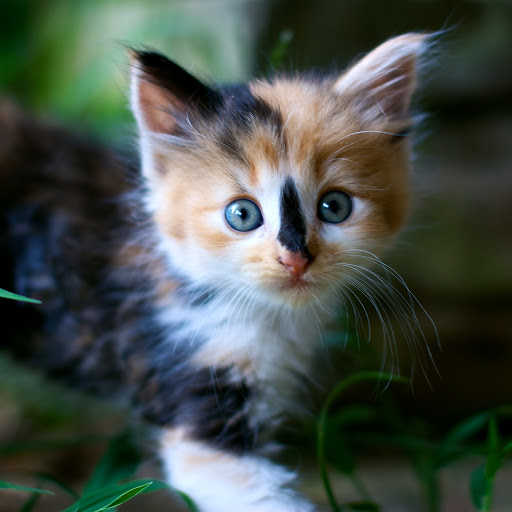
\includegraphics[width=\textwidth]{pictures/kitten.jpg}
		\caption[Original resolution photograph of a kitten]{Original $512\times512$ pixels photograph of a kitten \cite{travers_2009}}\label{fig:lennaoriginal}
	\end{minipage}
	\hfill
	\begin{minipage}[b]{0.45\textwidth}
		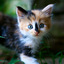
\includegraphics[width=\textwidth]{pictures/KittenDown.jpg}
		\caption[Reduced resolution photograph of a kitten]{Down-sampled $64\times64$ pixels photograph of a kitten}\label{fig:lennareduced}
	\end{minipage}
\end{figure}

Often, dimensionality reduction techniques are used to learn latent variables, which  are variables that are not directly observed. For example, in a picture of a kitten, a latent variable might be the cuteness of a kitten. Cuteness is not something that can be directly observed. A kitten can be observed to have a certain length of fur, a certain color of fur, eye diameter to head ratio, etc. but it is difficult to quantify a kitten's cuteness numerically. Whereas humans are able to claim a kitten is cute and can have a general consensus on it after looking at an image of a kitten, a machine might be able to learn what cuteness is by reducing the dimensionality of data and understanding it at a lower dimensional level but at a higher level of abstraction. These latent variables, along with other variables, can be used as input features to another machine learning algorithm which could be used learn more about the data. Hence, dimensionality reduction leads to feature extraction and feature engineering, the processes of finding important variables derived directly or indirectly from raw input. Generally, the set of features that arise from feature extraction and engineering can form what is called a latent space (also called feature embedding, embedding space or latent space). The latent space is able to represent data that may have originally been incomparable by a machine as comparable data points.
\subsection{Parametric Modeling and Optimization}
\label{paramsmodeling}

Although the different types of learning methods have been described, we still need a way to train these models. One way to do this is to restrict our function $f$ representing the machine learning algorithm to a function that is parametric and differentiable. By changing the parameters of the function, we hope to make it better in the task that we designed it for. Therefore, we augment our original functional form of our machine learning model, $\mathbf{\hat{y}} = f(\mathbf{X})$, and refer to it as $\mathbf{\hat{y}} = f(\mathbf{X} \ | \ \boldsymbol{\theta})$  where $\boldsymbol{\theta}$ is a vector of parameters of the given function and $f$ is a differentiable function with respect to $\boldsymbol{\theta}$. Hence, our goal would be to find a $\boldsymbol{\hat{\theta}}$ that minimizes the loss function, $J(\mathbf{y}, f(\mathbf{X} \ | \ \boldsymbol{\theta}))$. The best way to approach this problem would be to calculate the gradient with respect to $\boldsymbol{\theta}$, set it equal to zero and solve for a $\boldsymbol{\hat{\theta}}$ like so

\begin{equation}
	\nabla_{\boldsymbol{\theta}} J(\mathbf{y}, f(\mathbf{X} \ | \ \boldsymbol{\theta})) = 0.
\end{equation}

However, in many cases, it is either not possible to find a closed form solution or the way to do so becomes intractable, especially when the training set is large. Often, the gradient calculation with respect to the model's parameters are estimated and are not exact. Hence, instead of attempting to find an analytic solution, we must use gradient descent, a numerical optimization algorithm, by finding the direction of steepest descent and moving the parameters in that direction in the following way 

\begin{equation}
	\label{eq:sgd}
	\boldsymbol{\theta}_{t+1} \leftarrow \boldsymbol{\theta}_t - \eta \ \nabla_{\boldsymbol{\theta}} J(\mathbf{y}, f(\mathbf{X} \ | \ \boldsymbol{\theta})) 
\end{equation}

\noindent
where $\eta$ is the learning rate hyperparameter that controls the size of the step towards the direction of steepest descent as described by \citet{gd_explanation}. If this parameter is too large, the step towards $\boldsymbol{\hat{\theta}}$ will overshoot, miss $\boldsymbol{\hat{\theta}}$ and never converge. If this parameter is too small, the step towards $\boldsymbol{\hat{\theta}}$ will be more precise, but the time to find $\boldsymbol{\hat{\theta}}$ will be large. One way to solve this problem is to change the learning rate over time so that in the beginning large steps are taken and when the amount of change in between $\boldsymbol{\theta}_{t}$ and $\boldsymbol{\theta}_{t+1}$ is small, the learning rate is decreased as proposed by \citet{decreasing_learning_rate} in order to get as close to the optimum solution as possible. Gradient descent is the name that is usually given to the algorithm which calculates the gradient based on the entire training set and updates the parameters using that gradient value. Another form of gradient descent, stochastic gradient descent (SGD\nomenclature{SGD}{Stochastic Gradient Descent}) developed by \citet{sgd1} and \citet{sgd2}  calculates the gradient either for a single sample or a small batch of samples and takes small steps towards the optimal solution. SGD is computationally faster. Since large datasets cannot be held in RAM, it is faster to select mini-batches of data from the training set and calculate the gradient on said mini-batches. SGD is able to make more updates over a time period than gradient descent and results in a model as good as or better than that of gradient descent. Generally, this process is repeated multiple times on the training data and each repetition is called an \textit{epoch}.

Unfortunately, as the number of parameters that the equation needs to train increases, the classic SGD algorithm becomes insufficient. The algorithm finds parameters which are local minimums in the function $J$ as opposed to global minimums. An example of a global minimum and local minimum is shown in \cref{fig:minmax}. Consequently, the model that results is not as optimal as it can be. More sophisticated algorithms have been developed over time. One of these algorithms is called Adam and was developed by \citet{kingma2014adam}. 

\begin{figure}[!ht]
	\centering
	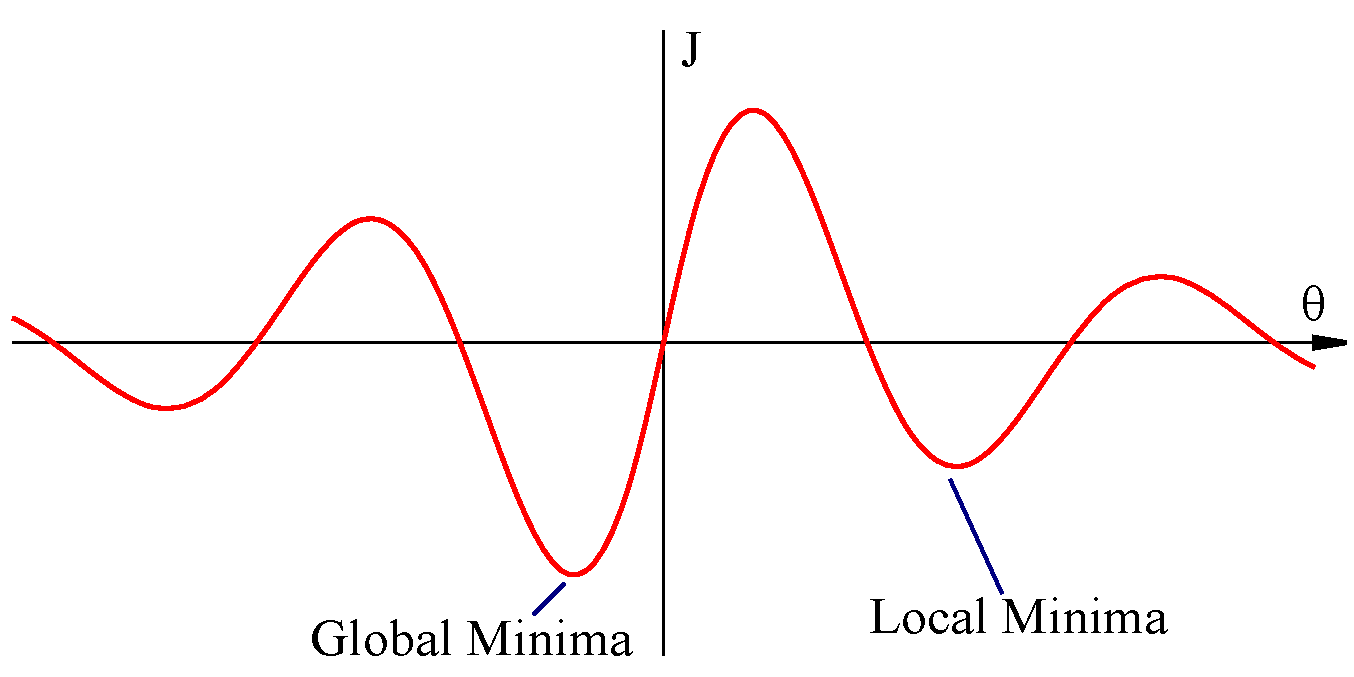
\includegraphics[width=0.6\linewidth]{pictures/minmax.pdf}
	\caption{Illustration of global minimum vs. local minimum}\label{fig:minmax}  
\end{figure}

Adam, the short form for Adaptive Moment Estimation, is a first-order optimization algorithm that uses running averages of the gradient as well as the  bias-corrected estimates to update the first two moments of the gradient to update $\boldsymbol{\theta}$. Moments are the measures of how the gradient has changed over the last couple of iterations,  The moment allows the optimization algorithm to act like a ball on a hill trying to roll to the lowest height possible. The ball will continue to roll even if a local minimum is achieved and continue to try to find a global minimum. In the case that the minimum that it finds \textit{is} the global minimum, the ball will continue to oscillate around that point until it loses momentum. Adam works in an analogous way. Therefore, we use Adam in our experiments as opposed to classic SGD for optimizing our models. 

\subsection{Bias-Variance Trade-off}
\label{bias_variance_tradeoff}

One of the main goals of machine learning is to learn a general trend from a limited amount of sample data. In other words, we expect training accuracy, i.e. the predictive accuracy of the model on the training set, and the testing accuracy, i.e. the predictive accuracy of the model on unseen data from the real world, to be as close as possible. Unfortunately, this is not always the case. \Cref{fig:overfit} demonstrates this concept by fitting a first and a twentieth-degree polynomial to the same data originating from a sinusoid using the least squares loss function given by \cref{eq:leastsquares}. 

\begin{equation}
	\label{eq:leastsquares}
	J(\mathbf{y}, f(\mathbf{X} \ | \ \boldsymbol{\theta})) = \sum_{i=0}^{N} (\mathbf{y}_i  - f(\mathbf{X} \ | \ \boldsymbol{\theta}_i))^2
\end{equation}


It is evident from \cref{fig:overfit} that the twentieth-degree polynomial tries to go through as many points as possible and ends up over-fitting the data. On the other hand, the first-degree polynomial tries to best fit the data but is unable to do so due to the lack of complexity and, therefore, under-fits the original data. Neither of these graphs represents the true nature of the sinusoid. Therefore, we are faced with a trade-off between two sources of errors: bias and variance. 

\begin{figure}[!ht]
	\centering
	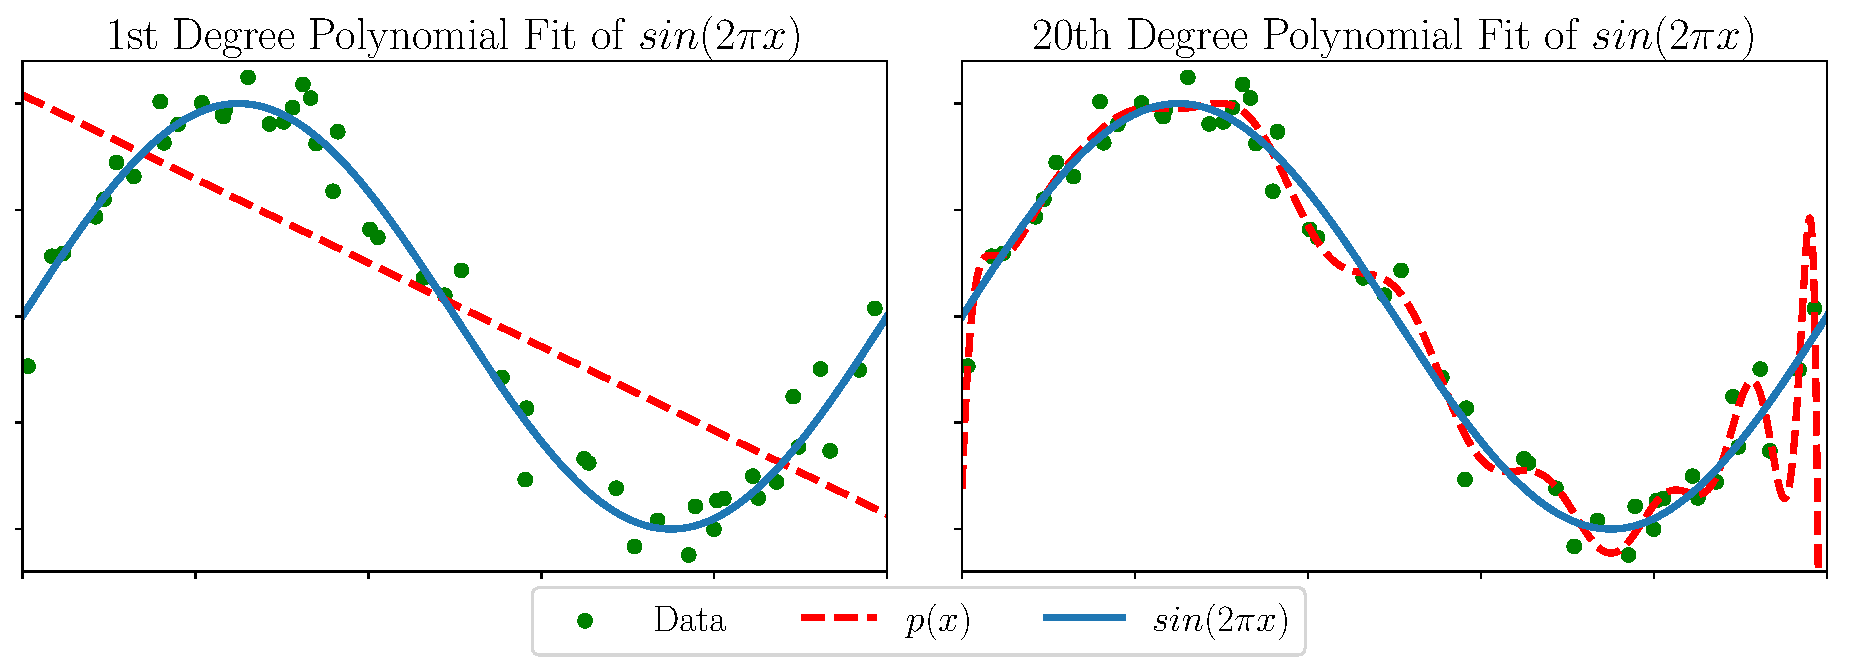
\includegraphics[width=\linewidth]{pictures/poly_fit.pdf}
	\caption[Example of an under-fit and an over-fit model]{Example of an under-fit (left) and an over-fit (right) model}\label{fig:overfit}  
\end{figure}

Bias is the error that arises from making overly simplistic assumptions about the underlying trend in the data and results from using too few parameters in the model we are training. Variance is the error that arises from making overly complicated assumptions about the underlying trend in the data and results from using too many parameters in the model we are training. These two errors comprise the bias-variance trade-off. In order to minimize this error, we need to make a compromise between these two sources of error and select a model that is neither complex nor simple.

\begin{figure}[!ht]
	\centering
	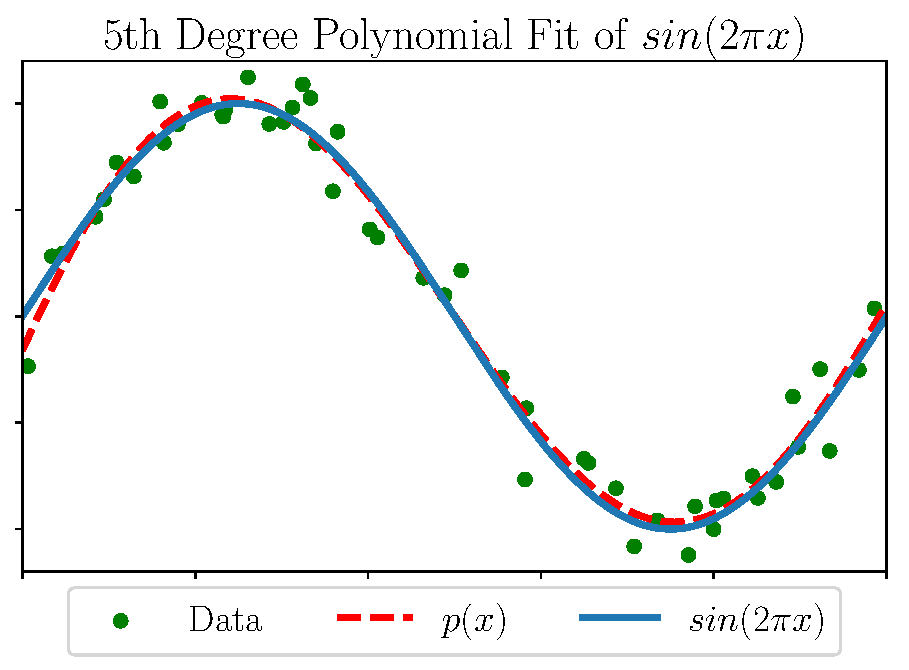
\includegraphics[width=0.5\linewidth]{pictures/poly_fit_correct.pdf}
	\caption{Example of a well-fit model}\label{fig:wellfit}  
\end{figure}

There are two ways that we can approach this problem. Either we can start with a simplistic model and make it more complex or we can start with a complex model and make it simpler. The latter is easier and the general name given to the process of making a relatively complex model simpler is called regularization. An example of a well-fit polynomial fit after simplifying the twentieth-degree polynomial is shown in \cref{fig:wellfit}.

In order for regularization to work, we need to know whether the model is generalizing well or not. Hence, we split the original training set, $\mathcal{S}$ into two mutually exclusive sets $\mathcal{S}_t$, the training set the model uses to learn, and $\mathcal{S}_v$, the validation set which we can use to see if the model is generalizing well to data that it has not seen before. If the validation accuracy is significantly lower than the training accuracy, we can infer that the model is not generalizing well.

One way we can regularize the model is by adding a penalty term to the loss function, $J(\mathbf{y}, f(\mathbf{X} \ | \ \boldsymbol{\theta}))$, based on the values of $\boldsymbol{\theta}$. The resulting loss function would then be

\begin{equation}
	J_{t}(\mathbf{y}, f(\mathbf{X} \ | \ \boldsymbol{\theta})) = J(\mathbf{y}, f(\mathbf{X} \ | \ \boldsymbol{\theta})) + \lambda \ P(\boldsymbol{\theta})
\end{equation}

\noindent
where $\lambda$ is a hyperparameter that controls how much we want to penalize a complex model and $P$ is a function such that $P(\boldsymbol{\theta}) \rightarrow \infty \text{ as } \theta_i \rightarrow \infty$. The two equations shown below are examples of such penalties. 


\begin{equation}
	\label{eq:l1}
	P(\boldsymbol{\boldsymbol{\theta}}) = \sum_{k = 1}^{N}{|\theta_k|}
\end{equation}

\begin{equation}
	\label{eq:l2}
	P(\boldsymbol{\theta}) = \sum_{k = 1}^{N}{\theta_k^2}
\end{equation}


\Cref{eq:l1} is known as the $L_1$ penalty and promotes sparsity. This means that the penalty forces any parameter that does not contribute to the model to zero thereby reducing the total number of parameters involved in the model. $L_2$ penalty, shown in \cref{eq:l2}, on the other hand, minimizes the contribution of a parameter but it does not force it to zero. Therefore, the number of parameters tends to be high, but the overall complex nature of the model is reduced. It is important to tune the hyperparameter $\lambda$ based on validation results in order to accurately penalize complex models to find a trade-off between bias and variance. 


\section{Neural Networks and Deep Learning}

Artificial Neural Networks (ANNs\nomenclature{ANN}{Artificial Neural Network}), also called neural networks, are a type of computational system that was originally inspired by biological neural networks found in organisms that have a nervous system. Neural networks are at the cutting edge of difficult machine learning tasks and have surpassed human-level performance in these tasks. Neural networks have been used to solve a variety of problems including those in computer vision, speech recognition, machine translation, video game bots and medical diagnostics \cite{imagenet_cnn,acoustic_modeling_speech,neural_translation,atari_deep_reinforcement_learning,3d_conf_for_alzheimers}.

\subsection{Motivation for Neural Networks}

Neural networks were originally inspired by biological neurons. Biological neurons generally consist of a cell body, dendrites, synapses and an axon. A dendrite is a part of a neuron that receives signals from other cells, including neurons, which were transmitted through a synapse as a chemical signal. These received signals are then propagated towards the cell body as an electrical signal. Once the cell body receives this electrical signal, more reactions happen within the cell body. If a certain action potential is reached, the neuron that received the signal fires and propagates the received signal along its axon towards other neurons and cells. A figure of a biological neuron is shown below in \cref{fig:bioneuron}. The biological nervous system is, in essence, a network of these cells interconnected with each other in various ways. 

\begin{figure}[!ht]
	\centering
	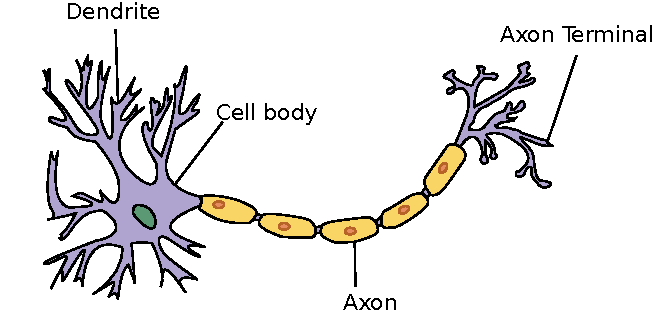
\includegraphics[width=0.7\linewidth]{pictures/Neuron.pdf}
	\caption[Illustration of a biological neuron]{Illustration of a biological neuron\cite{wiki:neuronpic}}\label{fig:bioneuron}  
\end{figure}

An artificial neural network tries to mimic a nervous system through the simulation of neurons. A visual representation of a single artificial neuron or node is shown in \cref{fig:activationblockdiagram}.  The inputs, $\{x_1 ... x_n\}$, are the set of numbers either given directly to the neuron or resulting from other neurons in the network. The neuron then multiplies each of these inputs by a corresponding weight $\{w_1 ... w_n\}$ and then sums these values together and adds a bias value $b$. The neuron then applies an activation function, $\sigma$, and delivers its result through its axon to the next neuron or neurons in the network. Types of activation functions are discussed in \cref{activationfunctions}. 

\begin{figure}[!ht]
	\centering
	\begin{tikzpicture}[
			init/.style={
				draw,
				circle,
				inner sep=2pt,
				font=\Huge,
				join = by -latex
			},
			squa/.style={
				regular polygon,
				regular polygon sides=4,
				draw,
				inner sep=0.3em,
				font=\Large,
				join = by -latex
			},
			start chain=2,node distance=13mm
		]
		\node[on chain=2] 
		(x2) {$x_2$};
		\node[on chain=2,join=by o-latex] (w2)
		{$w_2$};
		\node[on chain=2,init] (sigma) 
		{$\displaystyle + $};
		\node[on chain=2,squa,label=above:{\parbox{2cm}{}}]   
		{$\sigma$};
		\node[on chain=2,label=above:{},join=by -latex] 
		{$y$};
		\begin{scope}[start chain=1]
			\node[on chain=1] at (0,1.5cm) 
			(x1) {$x_1$};
			\node[on chain=1,join=by o-latex] 
			(w1) {$w_1$};
		\end{scope}
		\begin{scope}[start chain=3]
			\node[on chain=3] at (0,-1.5cm) 
			(xn) {$x_n$};
			\node[on chain=3,label=below:{},join=by o-latex] 
			(wn) {$w_n$};
		\end{scope}
		\node[label=above:\parbox{2cm}{\centering $b$}] at (sigma|-w1) (b) {};
																		
		\draw[-latex] (w1) -- (sigma);
		\path (x2) -- (xn) node [black, font=\large, midway, sloped] {$\dots$};
		\path (w2) -- (wn) node [black, font=\large, midway, sloped] {$\dots$};
		\draw[-latex] (wn) -- (sigma);
		\draw[o-latex] (b) -- (sigma);
																		
		(x1.north west) -- node[left=10pt] {Inputs} (xn.south west);
	\end{tikzpicture}
	\caption{Block diagram of a single artificial neuron}\label{fig:activationblockdiagram}  
\end{figure}

As described in \cref{paramsmodeling}, training a model is optimizing its learnable parameters, $\boldsymbol{\theta}$. The same concept applies to neural networks. The primary learnable parameters of the neural network are its weights. Depending on the architecture, i.e. the what parts the neural network is made up of, it may be possible to learn parameters presented in other parts of the neural network, such as the activation function. The process of learning any of these parameters for a neural network is called backpropagation. 

Backpropagation begins with the forward propagation of a set of inputs. Forward propagation is when a neural network infers the output for a particular set of inputs. The network propagates the inputs, $\mathbf{X}$, through each appropriate neuron in a neural network sequentially depending on the architecture until the propagation reaches the output neuron, which will result in $\mathbf{\hat{y}}$. The output neurons' results can be compared to the true output $\mathbf{y}$ and, unless the network is already trained, a significant amount of error is expected between $\mathbf{y}$ and $\mathbf{\hat{y}}$, which can be quantified by a loss function, $J(\mathbf{\hat{y}}, \mathbf{y})$. A large loss indicates that the parameters need to be optimized which means that each of the unoptimized parameters contributes a small error to the total error in the output. Therefore, we need to trace back the steps in the neural network and find the amount of error that each weight contributes for each input sample and adjust the respective weights. In other words, we are propagating the error backward towards every learnable parameter in the network, which is essentially the gradient of the loss function. Hence, \cref{eq:sgd} can be used to train the network. 


\subsection{Fully Connected Feed-Forward Networks}

A fully connected neural network (FC network\nomenclature{FC}{Fully Connected Neural Network}) is a neural network that propagates a signal layer by layer. The first layer in a neural network is commonly called the input layer since all the activations are inputs given to the network by the user. Depending on what the neural network is being used for, any of the next layers can be considered an output layer. In general, the last layer is considered the output layer. Any node not in either the input layer or the output layer are considered hidden nodes since these nodes' values do not matter to the input or the output; they are simply nodes that transfer information to the next layer or the next node. The neural network is considered to be a feed-forward network because the network does not propagate the information backward to previous nodes for any feedback. \Cref{fig:mlpillustrated} shows an illustration of a four-layer, fully connected, feed-forward neural network. The input layer contains four input nodes, both hidden layers contain five hidden nodes and the output layer contains three output nodes. The number of hidden layers and the number of nodes in each hidden layer are considered to be hyperparameters, parameters that can be controlled by the developer.

\def\layersep{2.5cm}
\def\finallayersep{7.5cm}
\def\hblayersep{5.0cm}
\begin{figure}[!ht]
	\centering
	\begin{tikzpicture}[shorten >=1pt,->,draw=black!50, node distance=\layersep]
		\tikzstyle{every pin edge}=[<-,shorten <=1pt]
		\tikzstyle{neuron}=[circle,draw=black!50,fill=none,minimum size=20pt,inner sep=5pt]
		\tikzstyle{input neuron}=[neuron];
		\tikzstyle{output neuron}=[neuron];
		\tikzstyle{hidden neuron}=[neuron];
		\tikzstyle{annot} = [text width=4em, text centered]
																		
		% Draw the input layer nodes
		\foreach \name / \y in {1/1,2/2.2,3/3.4,4/4.6}
		% This is the same as writing \foreach \name / \y in {1/1,2/2,3/3,4/4}
		\node[input neuron] (I-\name) at (0,-\y) {$ x_\name $};
																		
		% Draw the hidden layer nodes
		\foreach \name / \y in {1/1,2/2.2,3/3.4,4/4.6,5/5.8}
		\path[yshift=0.5cm]
		node[hidden neuron] (H-\name) at (\layersep,-\y cm) {};
																		
																		
		\foreach \name / \y in {1/1,2/2.2,3/3.4,4/4.6,5/5.8}
		\path[yshift=0.5cm]
		node[hidden neuron] (H2-\name) at (\hblayersep,-\y cm) {};
																		
		% Draw the output layer node
																		    
		\foreach \name / \y in {1/1,2/2.2,3/3.4}
		\path[yshift=-0.75cm]
		node[output neuron](O-\name) at (\finallayersep, -\y cm) {$y_\name$};
																		
		% Connect every node in the input layer with every node in the
		% hidden layer.
		\foreach \source in {1,2,3,4}
		\foreach \dest in {1,2,3,4,5}
		\path (I-\source) edge (H-\dest);
																		            
		\foreach \source in {1,2,3,4,5}
		\foreach \dest in {1,2,3,4,5}
		\path (H-\source) edge (H2-\dest);
																		
		% Connect every node in the hidden layer with the output layer
																		    
		\foreach \source in {1,2,3,4,5}
		\foreach \dest in {1,2,3}
		\path (H2-\source) edge (O-\dest);
																		
		% Annotate the layers
		\node[annot,above of=H-1, node distance=1.5cm] (hl) {Hidden layer 1};
		\node[annot,above of=H2-1, node distance=1.5cm] (hb) {Hidden layer 2};
		\node[annot,left of=hl] {Input layer};
		\node[annot,right of=hb] {Output layer};
	\end{tikzpicture}
									
	\caption{Graph diagram of a four-layer neural network}\label{fig:mlpillustrated}  
\end{figure}

Fully connected feed-forward networks can be easily represented in mathematics as a series of matrix multiplications and activation functions. If there are $K$ layers in this type of neural network, there will be $K-1$ weight matrices and $K-1$ bias vectors. Each weight matrix will have an entry for a weight from a neuron in the previous layer to a neuron in the current layer. In other words, if there are $N$ neurons in the previous layer and $M$ neurons in the current layer, there will be $N \times M$ entries in the weight matrix and $1 \times M$ entries in the bias vector. For example, the output of the neural network shown in \cref{fig:mlpillustrated} will be 

\begin{equation}
	\mathbf{\hat{y}} = \sigma(\sigma(\sigma(\mathbf{x} \times \mathbf{W_1} + \mathbf{b_1}) \times \mathbf{W_2} + \mathbf{b_2}) \times \mathbf{W_3} + \mathbf{b_3})
\end{equation}

\noindent
where $\sigma$ is the activation function that acts on a matrix entry by entry, $ \mathbf{x} \in \mathbb{R}^{1 \times 4} $ for an input with one sample, $\mathbf{W_1} \in \mathbb{R}^{4 \times 5}$, $\mathbf{b_1} \in \mathbb{R}^{1 \times 5}$, $\mathbf{W_2} \in \mathbb{R}^{5 \times 5}$, $\mathbf{b_2} \in \mathbb{R}^{1 \times 5}$,  $\mathbf{W_3} \in \mathbb{R}^{5 \times 3}$, and $\mathbf{b_3} \in \mathbb{R}^{1 \times 3}$. 

Backpropagation can be easily calculated for a simple FC network as demonstrated by \citet{ai_text_book}. 


\subsection{Convolutional Neural Networks}
\label{cnns}

Convolutional neural networks (CNNs\nomenclature{CNN}{Convolutional Neural Network}) are a class of networks that have been successful in the field of image processing. 

CNNs were also inspired by the biology of creatures that have vision. In $1965$, \citet{receptive_field} showed that cats contain neurons that respond to small regions of the field of vision. Assuming that the eyes are not moving, the concept of a receptive field, the particular region of vision that causes a single neuron to fire, was introduced. The concept of a receptive field is what led to what we know as a CNN.

CNNs attempt to learn shift-invariant characteristics in an input based on kernels, also called filters, which slide through the image and results in a filtered version of the original input image. The convolution computes the inner product of the kernel and the corresponding receptive field, saves the result to a new matrix known as the feature map, strides a particular length, and repeats the process until the entire input is convolved with the filter. \Cref{fig:convolution} shows an example of this process. The $3 \times 3$ kernel shown can be visualized as sliding over the input image represented as a $5\times5$ matrix. Note that a zero padding has been applied to the matrix so that the resulting feature map is the same size as the original image. However, it is also possible to forgo the padding and have the convolution result in a smaller sized feature map depending on the architecture of the neural network. The feature map is the result of the convolution and helps the network understand abstract patterns in the input, such as edges in the case of an image.   

\begin{figure}[!ht]
	\centering
	\begin{tikzpicture}
		\matrix (mtr)[matrix of nodes,nodes={inner sep=0pt,text width=0.8cm,align=center,minimum height=0.8cm, draw}]
		{
			0 & 0   & 0   & 0   & 0   & 0  & 0 \\
			0 & 0   & 21  & 0   & 0   & 0  & 0 \\
			0 & 85  & 71  & 0   & 0   & 0  & 0 \\
			0 & 250 & 231 & 127 & 63  & 3  & 0 \\
			0 & 250 & 252 & 250 & 209 & 56 & 0 \\
			0 & 250 & 252 & 250 & 250 & 83 & 0 \\
			0 & 0   & 0   & 0   & 0   & 0  & 0 \\
		};
																		    
		\node [below= 0.1cm of mtr-7-4.south] (lm) {$\bf Image$};
		\node [right= 3.5cm of lm] (km) {$\bf Kernel$};
		\node [right= 1.95cm of km] (km) {$\bf Feature \ Map$};
																		    
		\draw[very thick, red] (mtr-1-1.north west) rectangle (mtr-3-3.south east);
																		    
		\draw [ultra thick, fill=yellow, opacity=0.2] (mtr-2-2.north west) rectangle (mtr-6-6.south east);
																		
		\draw[line width=0.5mm, blue] (mtr-1-2.north west) rectangle (mtr-3-4.south east);
																		
		\node[right = 0.2em of mtr] (str) {$\ast$};
																		
		\matrix (K) [right=0.2em of str, matrix of nodes, nodes={inner sep=0pt,text width=0.8cm,align=center,minimum height=0.8cm, draw}]
		{
			0 & 0 & 1 \\
			0 & 1 & 0 \\
			1 & 0 & 0 \\
		};
																		
																		
		\node [right = 0.2em of K] (eq) {$=$};
		\matrix (ret) [right=0.2em of eq, matrix of nodes,nodes={inner sep=0pt,text width=0.8cm,align=center,minimum height=0.8cm, draw}]
		{
			0 & 106 & 71 & 0 & 0 \\
			106 & 321 & 231 & 127 & 63 \\
			321 & 481 & 379 & 313 & 212 \\
			481 & 629 & 565 & 462 & 306 \\
			502 & 502 & 459 & 306 & 83 \\
		};
																		
		\draw[very thick, red] (ret-1-1.north west) rectangle (ret-1-1.south east);
																		
		\draw[ultra thick, blue] (ret-1-2.north west) rectangle (ret-1-2.south east);
																		    
		\node[anchor=south east, inner sep=0.01em, purple] at (mtr-1-2.south east) (xx) {\scalebox{.7}{\hspace{-1.5em}$\times 0$}};
		\node[anchor=south east, inner sep=0.01em, purple] at (mtr-1-3.south east) (xx) {\scalebox{.7}{\hspace{-1.5em}$\times 0$}};
		\node[anchor=south east, inner sep=0.01em, purple] at (mtr-1-4.south east) (xx) {\scalebox{.7}{\hspace{-1.5em}$\times 1$}};
		\node[anchor=south east, inner sep=0.01em, purple] at (mtr-2-2.south east) (xx) {\scalebox{.7}{\hspace{-1.5em}$\times 0$}};
		\node[anchor=south east, inner sep=0.01em, purple] at (mtr-2-3.south east) (xx) {\scalebox{.7}{\hspace{-1.5em}$\times 1$}};
		\node[anchor=south east, inner sep=0.01em, purple] at (mtr-2-4.south east) (xx) {\scalebox{.7}{\hspace{-1.5em}$\times 0$}};
		\node[anchor=south east, inner sep=0.01em, purple] at (mtr-3-2.south east) (xx) {\scalebox{.7}{\hspace{-1.5em}$\times 1$}};
		\node[anchor=south east, inner sep=0.01em, purple] at (mtr-3-3.south east) (xx) {\scalebox{.7}{\hspace{-1.5em}$\times 0$}};
		\node[anchor=south east, inner sep=0.01em, purple] at (mtr-3-4.south east) (xx) {\scalebox{.7}{\hspace{-1.5em}$\times 0$}};
																		
	\end{tikzpicture}
	\caption{Illustration of a spatial convolution used in CNNs}\label{fig:convolution}  
\end{figure}
There are a few advantages in using CNNs over more traditional methods of image processing or FC networks. Suppose we are trying to classify the digits found in the MNIST dataset. Traditionally, a human is involved, hand-engineers filters that seem to work, and uses post-processing algorithms, which looks at the filtered image to finally classify it as a digit between zero to nine. However, the usage of neural networks, especially CNNs, has eliminated the need for hand engineering filters. Backpropagation has the ability to learn the weights just like it has the ability to learn the weights of a FC network. However, learning the weights of CNNs still take a long time due to the current hardware capabilities. The inference time of CNNs is also generally longer thant hat of traditional algorithms. Hence, if time is not of the essence, CNNs tend to be better than classical algorithms for image processing tasks.

It is also better to use CNNs over FC networks for a task where spatially invariant features may be involved. Assume again that we are trying to classify the digits found in the MNIST dataset. In a single digit, there are $28 \times 28$ pixels with values between $0$ to $255$. For a fully connected network, all of these pixels would be input nodes and therefore there would be $28 \times 28 = 784$ input neurons. Assuming that the first hidden layer has $250$ neurons, the weight matrix will have $784 \times 250 = 196000$ weights that will have to be trained. This is an enormous amount of weights for a relatively small input size. However, if we use a convolutional layer with $N$  $5 \times 5$ kernel on the same MNIST dataset, we would only have to train $N \times 25$ weights which means that the overall complexity of our network will go down and since we are learning a general trend, the average accuracy will go up. 

Series of convolutions can be placed sequentially after one another and gives the network a chance of learning more complicated spatial features that affect the final output. Networks that use series of convolutions one after another are commonly called deep convolutional neural networks or DCNNs\nomenclature{DCNN}{Deep Convolutional Neural Networks}. This is where the idea of deep learning arises since we are trying to increase the depth, the number of layers in a neural network, to learn more meaningful representations of data. 


\subsection{Pooling}
Pooling is a non-linear, sub-sampling operation in DCNNs which are used to reduce dimensions and the number of inputs to the subsequent layer. Pooling operations are non-parametric and they usually operate on the feature maps provided by convolutional layers before it. Two common types of pooling operations are used in neural networks: max-pooling and average pooling. Max-pooling \cite{scherer2010evaluation} finds the maximum element in a receptive field while average pooling takes the average of elements in the receptive field. Pooling is used in situations where the absolute location of features do not matter as much as the relative location of features.

\subsection{Dropout}
Dropout is a special type of regularization used in neural networks. The technique was motivated by the fact that both biological and artificial neurons make decisions based on the decisions of its predecessors. In the case that one of the predecessors of a particular neuron fires incorrectly, the current neuron is also more likely to fire incorrectly. In order to prevent this phenomenon, \citet{dropout} proposed this method of regularization which randomly zeros out a neuron's output based on a Bernoulli trial probability of $p$ for the current iteration of training. As a result, when a future neuron fires, its dependency on the previous neurons effectively decreases and has a better chance of learning a meaningful representation of the dataset. 


\subsection{Activation Functions}
\label{activationfunctions}

Several common activation functions are used today in cutting edge deep learning work. Our paper uses two of these activation functions: sigmoids and ReLUs. 
\subsubsection*{Sigmoid Activation}

The sigmoid activation has a functional form as follows: 

\begin{equation}
	\sigma(x) = \frac{1}{1 + exp(-x)}
\end{equation}

\noindent
and the corresponding gradient is 

\begin{equation}
	\sigma ' (x)  = \frac{exp(x)}{[exp(x) + 1]^2}.
\end{equation}. 

Brief analysis of the sigmoid's gradient shows that it suffers from the vanishing gradient problem, which refers to the function's gradient approaching zero as the input, $x$, increases or decreases. Because of this, sigmoid activations lead to extremely small gradient values and tend to slow down learning. However, sigmoids are very useful for final layers, especially in classification problems, since they limit output values to less than one. They are also commonly used in probability since the cumulative distribution function (CDF) of various probability distributions are sigmoidal in nature. As a result, the multi-dimensional analog of the sigmoid function, the softmax function, is used in neural network classification tasks to predict the probability that a given input is a particular class. 

\subsubsection*{ReLU}

Rectified Linear Units (ReLU\nomenclature{ReLU}{Rectified Linear Units}) have demonstrated performance increases in both accuracy, generalization and training speed in neural networks as shown by \citet{dahl2013improving}. ReLU has a functional form of:

\begin{equation}
	\rho(x) = max(x, 0)
\end{equation}

\noindent
and the corresponding gradient is 

\begin{equation}
	\rho'(x) =  \begin{cases} 
		
	0 & x \leq 0 \\
	1 & x > 0 \\
	\end{cases}.
\end{equation}

\noindent It is noticeable that the functional form of ReLU's gradient is a step function and only takes values of either 1 or 0. As a result, neurons with ReLU activations do not deal with the vanishing gradient or the exploding gradient problems as much as the sigmoid and speeds up the overall learning process. 

\section{Basics About EEG Signals}

The brain and the nervous system function on the basis of electrochemical reactions through biological neurons, as illustrated \cref{fig:bioneuron}, to send various signals to cells all over the body. Electroencephalography or EEG is a non-invasive way of measuring that electrical activity resulting on the surface of the brain due to these neurons. These signals can be used to diagnose seizures, brain tumors, head injuries, strokes, anesthesia overdose and many more ailments originating from the brain as described by \citet{mayo_eegs}.

According to \citet{eegs_info}, electrodes that measure voltage with respect to ground are attached to certain locations on the scalp as described by the $10$-$20$ system. An illustration of the $10$-$20$ system's placement map is shown in \cref{fig:tentwenty}. The letters and numbers on each of these electrodes can be used as an indication of location for each of the twenty-one channels in the EEG. 

\begin{figure}[!ht]
	\centering
	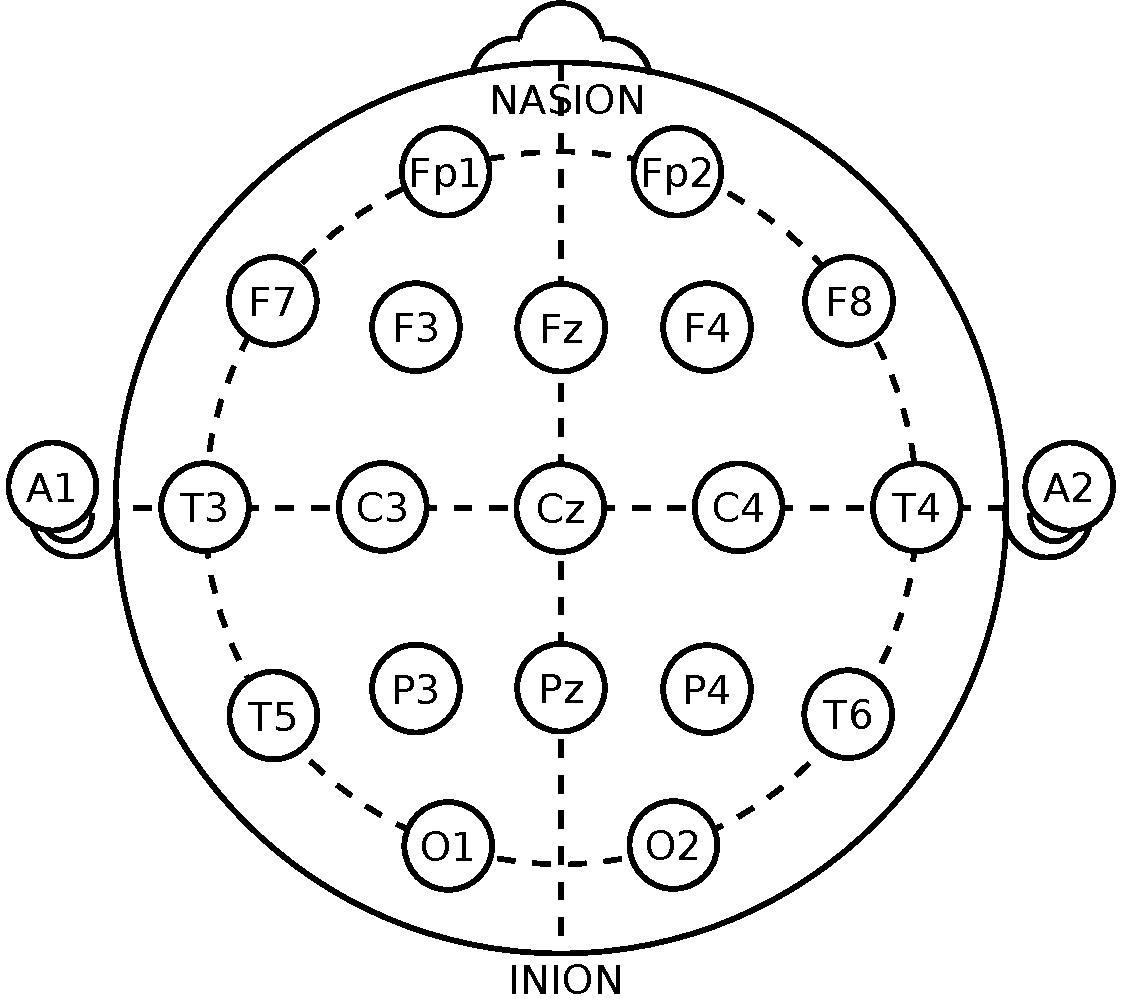
\includegraphics[height=0.45\linewidth]{pictures/tentwenty.pdf}
	\caption[Illustration of the $10$-$20$ system]{Illustration of the $10$-$20$ system used to place EEG electrodes provided by \citet{wiki:tentwenty}} \label{fig:tentwenty}
\end{figure}


Montages, voltage differences between certain probes, are used to extract information from these signals as opposed to the sole voltages sensed by the probes. Referential montages use the difference between a measuring electrode and a designated reference electrode. The reference electrode could be the ground which would mean the voltages sensed by the electrodes with respect to the ground can be used as the output of the EEG. In average reference montage, the outputs of all the electrodes are used as the reference voltage. Bipolar montages use the differences between two adjacent electrodes, e.g. F3 and C3 dubbed ``F3-C3'', as the output of the EEG. In Laplacian montages, the output is the voltage difference between an electrode and the average of the neighboring electrodes. 

A variety of different information can be extracted from these montages that can be used to classify the EEG activity. Frequency is one of these measurements. Rhythmic activity is considered to be constant in frequency, arrhythmic activity is where no rhythms are present, dysrhythmic activity is a pattern that is rarely seen in healthy subjects. Frequency is also generally classified as delta, theta, alpha or beta waves. Delta waves have a frequency of $3$Hz or below, theta waves have frequencies between $3.5$Hz to $7.5$Hz, alpha waves have frequencies between $7.5$Hz and $13$Hz, and beta waves have frequencies above $14$Hz. Generally, only waves between $0$Hz and $70$Hz are considered since the rest of the signal is considered to be high-frequency noise in most cases and can be ignored.

The amplitude of these signals also tends to be useful. When a person is awake, beta waves usually dominate EEGs meaning that the average amplitude of the signals are small and the frequency is high. As a person starts to close their eyes, the average amplitude increases and the frequency starts to drop resulting in alpha waves. When a person starts to sleep, theta waves dominate, the average amplitude increases and the frequency decreases. Finally, in deep sleep, delta waves are observed in normal patients, the amplitude is generally large and the signal has very low frequencies. Therefore, we can logically deduce some things about the patient using amplitude and frequency together.  Heuristically say that if a person's EEG contains high frequencies and high amplitudes, they may be experiencing a seizure. 

However, such simplistic heuristics cannot always be used to extract useful information from patients. Therefore,  a professional \textit{or} an algorithm that considers the complexity of EEGs needs extract meaningful, diagnostic information.